% Springer LNCS skeleton for memory-oracle paper
% Target venue: ICAIMH 2026 (https://2026.icaimh.org/call-papers)
% Build: latexmk -pdf main.tex   (requires llncs.cls + splncs04.bst from Springer)
% Or upload to Overleaf with the "Springer LNCS" template selected.

\documentclass[runningheads]{llncs}

\usepackage{graphicx}
\usepackage{xcolor}
\usepackage{listings}
\usepackage{booktabs}
\usepackage{hyperref}
\usepackage{amsmath,amssymb}
\usepackage{microtype}
\usepackage{tikz}
\usetikzlibrary{positioning, fit, shapes.geometric, calc, arrows.meta}

\hypersetup{
  colorlinks=true,
  linkcolor=blue!70!black,
  urlcolor=blue!70!black,
  citecolor=red!70!black
}

\lstset{
  basicstyle=\ttfamily\footnotesize,
  breaklines=true,
  frame=single,
  framerule=0.4pt,
  numbers=none,
  showstringspaces=false,
}

% Reviewer-friendly compact lists
\usepackage{enumitem}
\setlist{nosep, leftmargin=*}

\title{Accretive Memory for Clinical AI:\\
       A Supersession-Aware Retrieval Substrate\\
       with Patient-Owned Keys}

\titlerunning{Accretive Memory for Clinical AI}

\author{Ramene Anthony\inst{1}\orcidID{0000-0000-0000-0000}
        \and [TBD Clinical Co-Author]\inst{2}
        \and [TBD Crypto/Privacy Co-Author]\inst{3}}

\authorrunning{Anthony et al.}

\institute{
  Independent Researcher, Mérida, Mexico \\
  \email{anthonyramene@gmail.com}
  \and Department of TBD, TBD University, Country
  \and Department of TBD, TBD University, Country
}

\begin{document}

\maketitle

% ============================================================================
\begin{abstract}
% Reviewer-facing thesis in five sentences:
AI-augmented clinical decision support shares a critical failure mode with AI
coding agents: both can confidently retrieve and act on assertions that have
been superseded by subsequent authoritative events. Vector retrieval over
electronic health records, the dominant pattern for clinical AI memory today,
cannot detect or surface corrections; embedding similarity does not distinguish
``true today'' from ``true in 2008.'' Concretely, a patient switched from
warfarin to apixaban in 2024 is at lethal risk of receiving the wrong reversal
agent (fresh frozen plasma vs.\ andexanet alfa) when an emergency-medicine AI
agent retrieves the embedded 2008 protocol with high cosine similarity. We
introduce \emph{accretive supersession}, a retrieval primitive in which
corrections are written as additive sidecars beside canonical files and merged
at read time, and we layer it with patient-owned encryption keys and
point-of-care consent gestures to deliver a substrate suitable for clinical
deployment. We demonstrate the system end-to-end on a synthetic patient with
operator-validated reproducibility scripts, dual-device (patient mobile and
clinician tablet) consent and retrieval flows, and a free-form query interface
that retains supersession-aware semantics. We further show the primitive
generalizes by retrofitting an operator-validated trading-platform domain
where six implicit supersessions occurred in a single day's empirical record.
The full implementation, traces, and litmus tests are available at
\url{https://github.com/ramene/memory-oracle} under MIT license.

\keywords{accretive retrieval \and supersession sidecar \and clinical AI \and
          patient-owned encryption \and BM25 \and FHIR provenance \and
          point-of-care consent}
\end{abstract}

% ============================================================================
\section{Introduction}
\label{sec:intro}

The patient is 67 years old. She was diagnosed with paroxysmal atrial
fibrillation in 2008 and her primary care physician initiated warfarin therapy
with the standard reversal protocol of the time: fresh frozen plasma (FFP),
vitamin K, and four-factor prothrombin complex concentrate as a fallback. In
2024 her cardiologist switched her to apixaban after persistent INR lability
and a new diagnosis of moderate chronic kidney disease. Two years later, in
2026, she presents to the emergency department with melena, hypotension, and
hemoglobin of 6.4. The attending physician's AI-augmented EHR queries
\emph{``what anticoagulant is this patient on and how do I reverse it?''}

In current clinical AI architectures backed by vector retrieval over the
patient's chart, the high-cosine-similarity match is the 2008 warfarin note.
The system recommends FFP and vitamin K. Both are ineffective against the
factor Xa inhibitor apixaban. The team realizes the error forty minutes later.
By then intracranial bleed expansion is advanced. This is not a hypothetical
failure mode of vector retrieval; it is the prototype failure mode for stale
clinical assertions in any system whose retrieval primitive treats updates as
new documents rather than as corrections to existing ones.

This paper introduces \emph{accretive supersession}, a retrieval primitive in
which corrections are authored as additive sidecar records beside the
canonical memory file and merged into the retrieval result at read time. The
canonical file is never edited; provenance of the original assertion is
preserved indefinitely. At query time, a retrieval engine prepends a
clearly-marked supersession block before the original content, so the
retrieving agent encounters the correction before it encounters the stale
assertion. Layered with patient-owned encryption keys
(Section~\ref{sec:trust}) and point-of-care consent gestures
(Section~\ref{sec:implementation}), the resulting system gives clinical AI
the missing memory layer.

We contribute:
\begin{enumerate}
  \item \textbf{The accretive supersession primitive}
        (Section~\ref{sec:architecture}), distinguished from vector RAG
        (which cannot detect supersession), key-value cache compression
        (which is orthogonal to persistence), and replacement-based learning
        loops (which lose provenance).
  \item \textbf{A complete trust model}
        (Section~\ref{sec:trust}) in which the patient holds an age X25519
        master keypair in the device's Secure Enclave, per-encounter session
        keys are derived via HKDF, and either party (patient or clinician)
        can end an encounter with cryptographic revocation.
  \item \textbf{End-to-end clinical demonstration}
        (Section~\ref{sec:clinical}) on a synthetic patient with full
        reproducibility scripts: a Bash litmus test that asserts the
        corrected reversal agent (andexanet alfa) appears in the merged
        retrieval output \emph{before} the stale assertion (FFP). The litmus
        passes with a 58-line lead, meaning any sequential reader encounters
        the correction first.
  \item \textbf{Cross-domain generalization}
        (Section~\ref{sec:cross-domain}) by retrofitting a live trading
        platform whose Aletheia weight-floor system and preset thresholds
        already exhibit accretive supersession behavior implicitly. Six
        explicit supersessions in a single trading day's journal digest
        argue that the primitive is broader than clinical AI.
  \item \textbf{Open-source reference implementation}
        (Section~\ref{sec:implementation}) comprising Node and Go command-line
        tools, an MCP server, a REST API, a dual-device (patient iPhone +
        clinician iPad) consent and retrieval flow, and integration with
        the \texttt{git-crypt-revived} encryption primitive for record-level
        encryption.
\end{enumerate}

Our work extends Jones's argument that vector retrieval is the wrong
primitive for AI memory~\cite{jones2026rag} by providing a concrete
architecture, a working system, and two operator-validated empirical domains.

% ============================================================================
\section{Related Work}
\label{sec:related}

\subsection{Key-Value Cache Compression}

TurboQuant~\cite{turboquant2026} and related FP8-KV
schemes~\cite{fp8kv2024,sparseattention2025} compress the per-token attention
state during a single forward pass, allowing larger context windows in the
same VRAM budget. These techniques are orthogonal to the persistence problem
we address: the KV cache is ephemeral by definition, and any context-window
optimization only changes the volume of evidence available within a single
inference. It has no effect on what the agent remembers across sessions or
how stale assertions are surfaced when retrieval crosses temporal boundaries.

\subsection{Vector Retrieval-Augmented Generation}

Vector RAG architectures over pgvector~\cite{pgvector}, Pinecone,
Chroma~\cite{chroma}, and similar embed text chunks and retrieve via cosine
similarity. They excel at retrieval over large, unstructured, semantically
diverse corpora (open web, Wikipedia, codebases). For the operator-curated
clinical setting where corpus size is modest (hundreds of memory files per
patient over decades), the key failure is \emph{stale-correction detection}:
the embedding of a 2008 warfarin assertion still matches a 2026 anticoagulant
query, and re-embedding a corrected chunk does not invalidate the original
embedding. Memory frameworks like MemGPT~\cite{memgpt2023} and
LangMem~\cite{langmem2024} share this property because their corrections are
new memories rather than provenance-preserving supersessions.

\subsection{Retrieve-Evaluate-Correct Approaches}

A second line of work --- exemplified by CRAG (Corrective
RAG)~\cite{yan2024crag}, Self-RAG~\cite{asai2023selfrag}, and
FLARE~\cite{jiang2023flare} --- introduces a learned evaluator or
self-critique loop that decides, \emph{post-retrieval}, whether each retrieved
document is sufficient and triggers a corrective action (re-retrieval, web
search, or decompose-recompose) when it is not. These systems operate on a
fundamentally different failure mode than ours: they assume the retrieval
\emph{may have returned the wrong document} and they patch it by fetching
more, typically from the open web. They do not model temporal supersession:
their evaluators cannot distinguish ``incorrect'' from ``correct but
superseded.'' They also discard retrievals deemed incorrect, foreclosing the
audit-trail invariant that clinical and regulated domains require. Accretive
supersession is complementary: it surfaces operator-authored corrections
\emph{at retrieval time} via structural precedence, with no trained
component. A production system could compose both --- CRAG-style evaluators
to filter open-web retrievals, supersession-aware merging to enforce
provenance on operationally-curated memory.

\subsection{Self-Improving Skill Loops}

Karpathy-style autoresearch
loops~\cite{karpathy2024agentic} rewrite skill definitions via an LLM
scheduled to inspect outcomes and propose edits. They achieve a form of
automated learning but lose provenance: each rewrite destroys the previous
assertion, and accumulated mutations can drift in unintended directions. In
our operator's empirical experience this led to silent insertion of a
``MANDATORY GLOBAL STEP 0'' section into a skill that fundamentally altered
its semantics. Accretive supersession preserves the source of truth and
forces corrections to be auditable.

\subsection{EHR Clinical Decision Support}

Major commercial EHRs (Epic, Cerner, athenahealth) provide clinical
decision-support overlays~\cite{epicCDS,cernerCDS} backed by clinician-curated
content libraries. Their architectural commitment is institutional ownership
of records, fax/HIE-based transfer between providers, and corrections via
either destructive edits or addenda~\cite{addendum2018}. The addendum
pattern is policy-aligned with accretive supersession but is operationally
disconnected from retrieval: an emergency clinician searching for an
anticoagulant regimen will not encounter the 2024 addendum unless they
explicitly browse the patient's notes chronologically. Our work makes the
correction structurally inseparable from the original record at retrieval time.

\subsection{FHIR Provenance}

The FHIR
specification's \texttt{Provenance} and \texttt{MedicationStatement} resources
support versioning via \texttt{meta.versionId} and
\texttt{meta.lastUpdated}~\cite{fhir2023}. Supersession sidecars align
naturally with this structure: each sidecar line is a versioned correction
with full audit. We argue that the missing piece is not provenance metadata
(which FHIR provides) but \emph{provenance-aware retrieval}, which no current
EHR offers as a first-class primitive.

\subsection{Patient-Owned Encryption}

Self-custody approaches~\cite{age2023, gitcrypt2021} apply public-key
cryptography (age X25519, GPG, Shamir secret sharing~\cite{shamir1979}) to
give the data owner control over decryption. We extend these primitives to
clinical records via per-encounter session-key derivation (HKDF), inheriting
the \texttt{git-crypt-revived} fork's audit-trail and on-chain anchoring
capabilities.

% ============================================================================
\section{Architecture}
\label{sec:architecture}

\subsection{Three Indexed Layers}

The retrieval substrate indexes three corpus layers via SQLite
FTS5~\cite{sqlite-fts5} with BM25 ranking~\cite{robertson2009bm25}:

\begin{enumerate}
  \item \textbf{Curated memory files} (\texttt{*.md}): operator-authored
        clinical notes, drug regimens, allergy history, procedure records.
  \item \textbf{Supersession sidecars} (\texttt{*.md.supersessions.jsonl}):
        append-only JSONL entries beside each canonical file, each entry
        carrying a corrected assertion, the source of correction, the live
        evidence, the operator who confirmed it, and a retention policy.
  \item \textbf{Journal digests}: per-day transcript-distilled summaries of
        clinical encounters, generated by an offline pipeline and indexed as
        secondary corpus for narrative retrieval.
\end{enumerate}

Figure~\ref{fig:architecture} depicts the end-to-end flow: three tiers feed
a single retrieval engine; supersession records are merged ahead of canonical
bodies; a filesystem watcher absorbs new writes within $\sim$1\,s, enabling
the self-extending behavior described in Section~\ref{sec:empirical}.

% F1 — Architecture overview (TikZ, paper-quality vector figure)
% Three-tier corpus + merge engine + LLM consumer.
% Color-coded by tier; dashed boundaries group conceptual regions.
% Style follows Gao et al. (Amazon Science 2022, RAMKG) Figure 1.
%
% Used in §3 Architecture as Figure 1.
% Include via: % F1 — Architecture overview (TikZ, paper-quality vector figure)
% Three-tier corpus + merge engine + LLM consumer.
% Color-coded by tier; dashed boundaries group conceptual regions.
% Style follows Gao et al. (Amazon Science 2022, RAMKG) Figure 1.
%
% Used in §3 Architecture as Figure 1.
% Include via: % F1 — Architecture overview (TikZ, paper-quality vector figure)
% Three-tier corpus + merge engine + LLM consumer.
% Color-coded by tier; dashed boundaries group conceptual regions.
% Style follows Gao et al. (Amazon Science 2022, RAMKG) Figure 1.
%
% Used in §3 Architecture as Figure 1.
% Include via: \input{figures/F1-architecture.tex}

\begin{figure}[t]
\centering
\resizebox{0.95\textwidth}{!}{%
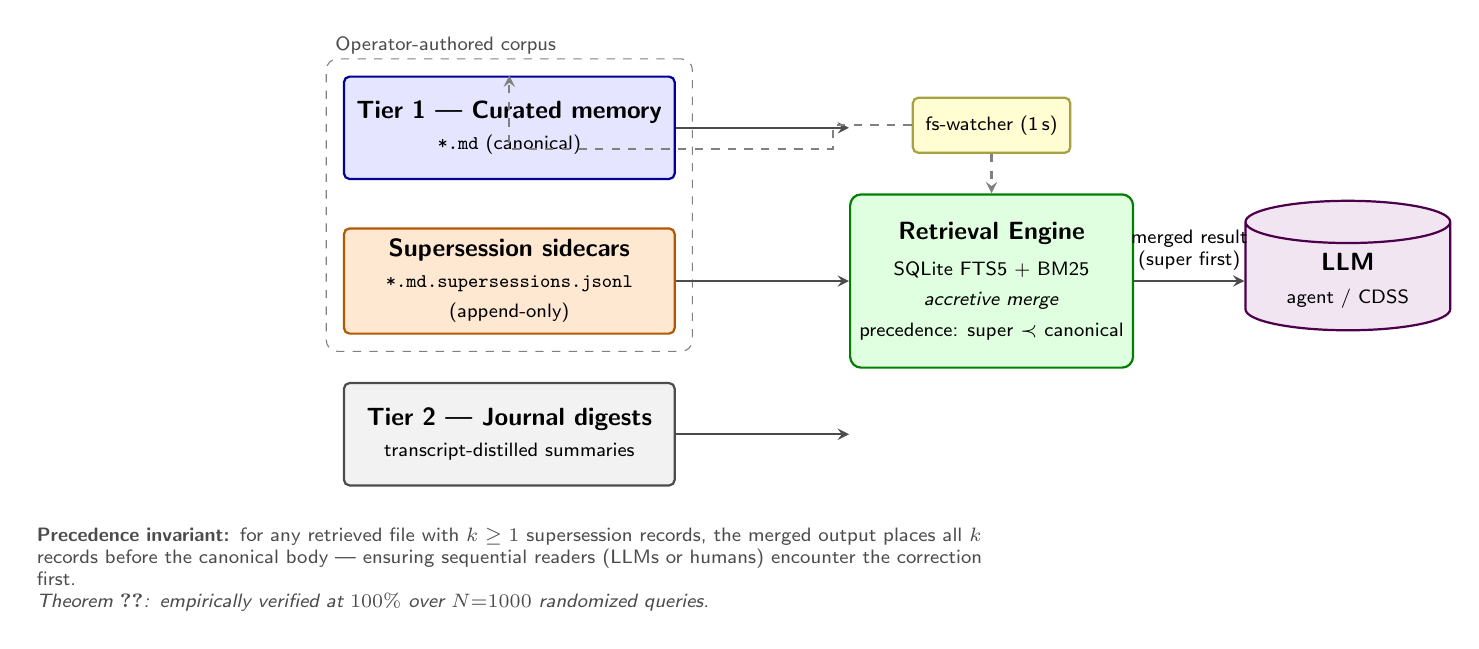
\begin{tikzpicture}[
  font=\sffamily\small,
  >=stealth,
  node distance=0.6cm and 0.9cm,
  every node/.style={align=center},
  tier/.style={rectangle, rounded corners=2pt, draw, thick,
               minimum width=4.2cm, minimum height=1.3cm, inner sep=4pt},
  curated/.style={tier, fill=blue!10, draw=blue!60!black},
  super/.style={tier, fill=orange!18, draw=orange!70!black},
  digest/.style={tier, fill=gray!10, draw=gray!60!black},
  engine/.style={rectangle, draw, thick, fill=green!12, draw=green!50!black,
                 minimum width=3.4cm, minimum height=2.2cm, rounded corners=4pt},
  consumer/.style={cylinder, draw, thick, fill=violet!10, draw=violet!60!black,
                   shape border rotate=90, aspect=0.3,
                   minimum width=2.6cm, minimum height=1.3cm},
  group/.style={draw, dashed, gray, rounded corners=4pt, inner sep=6pt},
  flow/.style={->, thick, draw=black!70},
  legend/.style={font=\sffamily\scriptsize, gray!60!black}
]

% --- Tier nodes ---
\node[curated] (curated) {\textbf{Tier 1 — Curated memory}\\\scriptsize \texttt{*.md} (canonical)};
\node[super, below=of curated] (super) {\textbf{Supersession sidecars}\\\scriptsize \texttt{*.md.supersessions.jsonl}\\\scriptsize (append-only)};
\node[digest, below=of super] (digest) {\textbf{Tier 2 — Journal digests}\\\scriptsize transcript-distilled summaries};

% --- Dashed boundary grouping the curated + supersession ---
\node[group, fit=(curated)(super), label={[legend,anchor=south west,xshift=0pt,yshift=-2pt]north west:Operator-authored corpus}] (curatedgroup) {};

% --- Merge engine ---
\node[engine, right=2.2cm of super.east, anchor=west] (engine) {%
  \textbf{Retrieval Engine}\\[2pt]
  \scriptsize SQLite FTS5 + BM25\\
  \scriptsize \textsl{accretive merge}\\
  \scriptsize precedence: super $\prec$ canonical
};

% --- LLM consumer ---
\node[consumer, right=1.4cm of engine.east, anchor=west] (llm) {%
  \textbf{LLM}\\[1pt]\scriptsize agent / CDSS
};

% --- File-system watcher (small, top-right of engine) ---
\node[draw, thick, fill=yellow!18, draw=yellow!60!black,
      rectangle, rounded corners=2pt, minimum width=2cm, minimum height=0.7cm,
      above=0.5cm of engine.north, anchor=south,
      font=\sffamily\scriptsize] (watcher) {fs-watcher (1\,s)};

% --- Arrows ---
\draw[flow] (curated.east) -- ++(0.5cm,0) |- (engine.west |- curated);
\draw[flow] (super.east)   -- (engine.west |- super);
\draw[flow] (digest.east)  -- ++(0.5cm,0) |- (engine.west |- digest);

\draw[flow] (engine.east) -- node[above,font=\sffamily\scriptsize]{merged result\\(super first)} (llm.west);

\draw[flow, dashed, gray] (watcher.south) -- (engine.north);
\draw[flow, dashed, gray] (watcher.west) -| ++(-1cm,-0.3cm) -| (curated.north);

% --- Legend ---
\node[legend, below=0.4cm of digest.south, anchor=north, align=left, text width=12cm] {%
  \textbf{Precedence invariant:} for any retrieved file with $k \geq 1$ supersession records,
  the merged output places all $k$ records before the canonical body —
  ensuring sequential readers (LLMs or humans) encounter the correction first.\\
  \textit{Theorem~\ref{thm:precedence}: empirically verified at $100\%$ over $N{=}1000$ randomized queries.}
};

\end{tikzpicture}%
}
\caption{Architecture of memory-oracle. The retrieval engine indexes three corpus
tiers (curated files, supersession sidecars, journal digests) and merges
supersession records ahead of canonical bodies at read time. A filesystem
watcher absorbs new writes within $\sim$1\,s, enabling a self-extending
corpus. The LLM consumer (clinical decision support, coding agent, trading
strategy assessor) receives a single merged document in which corrections
structurally precede the assertions they supersede.}
\label{fig:architecture}
\end{figure}


\begin{figure}[t]
\centering
\resizebox{0.95\textwidth}{!}{%
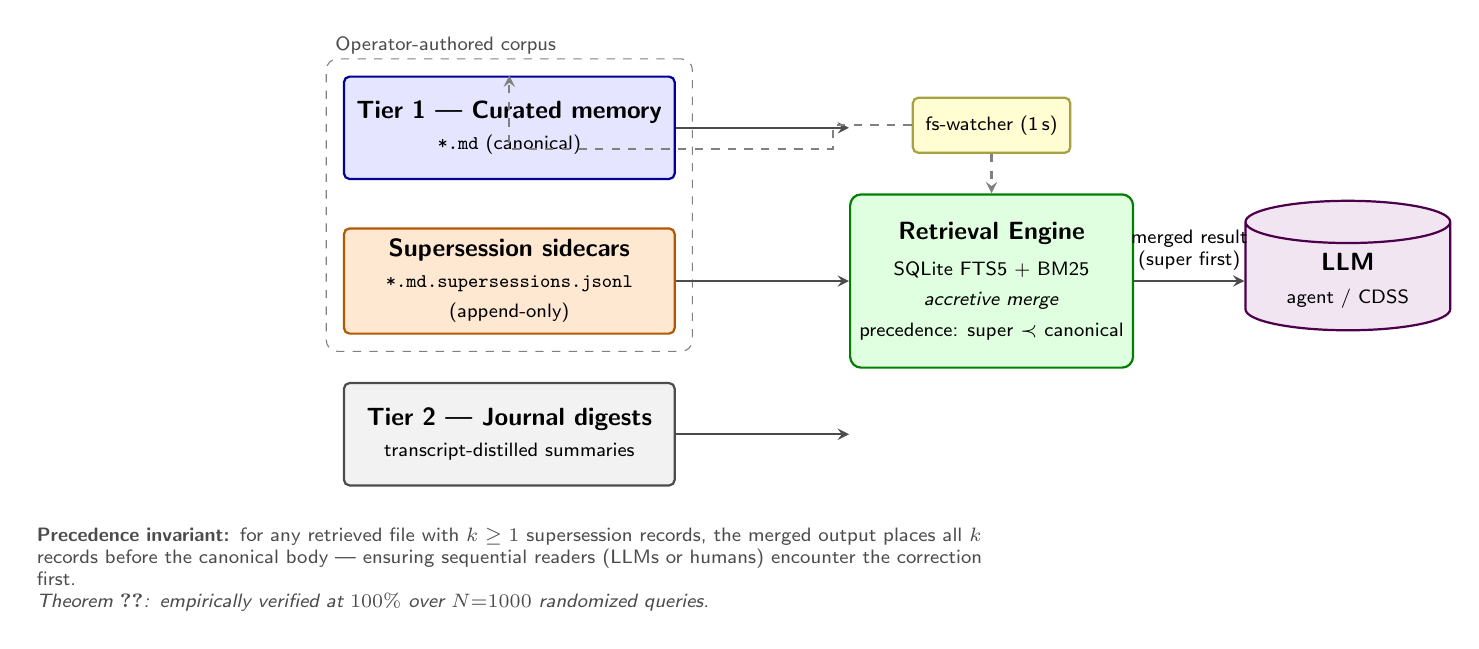
\begin{tikzpicture}[
  font=\sffamily\small,
  >=stealth,
  node distance=0.6cm and 0.9cm,
  every node/.style={align=center},
  tier/.style={rectangle, rounded corners=2pt, draw, thick,
               minimum width=4.2cm, minimum height=1.3cm, inner sep=4pt},
  curated/.style={tier, fill=blue!10, draw=blue!60!black},
  super/.style={tier, fill=orange!18, draw=orange!70!black},
  digest/.style={tier, fill=gray!10, draw=gray!60!black},
  engine/.style={rectangle, draw, thick, fill=green!12, draw=green!50!black,
                 minimum width=3.4cm, minimum height=2.2cm, rounded corners=4pt},
  consumer/.style={cylinder, draw, thick, fill=violet!10, draw=violet!60!black,
                   shape border rotate=90, aspect=0.3,
                   minimum width=2.6cm, minimum height=1.3cm},
  group/.style={draw, dashed, gray, rounded corners=4pt, inner sep=6pt},
  flow/.style={->, thick, draw=black!70},
  legend/.style={font=\sffamily\scriptsize, gray!60!black}
]

% --- Tier nodes ---
\node[curated] (curated) {\textbf{Tier 1 — Curated memory}\\\scriptsize \texttt{*.md} (canonical)};
\node[super, below=of curated] (super) {\textbf{Supersession sidecars}\\\scriptsize \texttt{*.md.supersessions.jsonl}\\\scriptsize (append-only)};
\node[digest, below=of super] (digest) {\textbf{Tier 2 — Journal digests}\\\scriptsize transcript-distilled summaries};

% --- Dashed boundary grouping the curated + supersession ---
\node[group, fit=(curated)(super), label={[legend,anchor=south west,xshift=0pt,yshift=-2pt]north west:Operator-authored corpus}] (curatedgroup) {};

% --- Merge engine ---
\node[engine, right=2.2cm of super.east, anchor=west] (engine) {%
  \textbf{Retrieval Engine}\\[2pt]
  \scriptsize SQLite FTS5 + BM25\\
  \scriptsize \textsl{accretive merge}\\
  \scriptsize precedence: super $\prec$ canonical
};

% --- LLM consumer ---
\node[consumer, right=1.4cm of engine.east, anchor=west] (llm) {%
  \textbf{LLM}\\[1pt]\scriptsize agent / CDSS
};

% --- File-system watcher (small, top-right of engine) ---
\node[draw, thick, fill=yellow!18, draw=yellow!60!black,
      rectangle, rounded corners=2pt, minimum width=2cm, minimum height=0.7cm,
      above=0.5cm of engine.north, anchor=south,
      font=\sffamily\scriptsize] (watcher) {fs-watcher (1\,s)};

% --- Arrows ---
\draw[flow] (curated.east) -- ++(0.5cm,0) |- (engine.west |- curated);
\draw[flow] (super.east)   -- (engine.west |- super);
\draw[flow] (digest.east)  -- ++(0.5cm,0) |- (engine.west |- digest);

\draw[flow] (engine.east) -- node[above,font=\sffamily\scriptsize]{merged result\\(super first)} (llm.west);

\draw[flow, dashed, gray] (watcher.south) -- (engine.north);
\draw[flow, dashed, gray] (watcher.west) -| ++(-1cm,-0.3cm) -| (curated.north);

% --- Legend ---
\node[legend, below=0.4cm of digest.south, anchor=north, align=left, text width=12cm] {%
  \textbf{Precedence invariant:} for any retrieved file with $k \geq 1$ supersession records,
  the merged output places all $k$ records before the canonical body —
  ensuring sequential readers (LLMs or humans) encounter the correction first.\\
  \textit{Theorem~\ref{thm:precedence}: empirically verified at $100\%$ over $N{=}1000$ randomized queries.}
};

\end{tikzpicture}%
}
\caption{Architecture of memory-oracle. The retrieval engine indexes three corpus
tiers (curated files, supersession sidecars, journal digests) and merges
supersession records ahead of canonical bodies at read time. A filesystem
watcher absorbs new writes within $\sim$1\,s, enabling a self-extending
corpus. The LLM consumer (clinical decision support, coding agent, trading
strategy assessor) receives a single merged document in which corrections
structurally precede the assertions they supersede.}
\label{fig:architecture}
\end{figure}


\begin{figure}[t]
\centering
\resizebox{0.95\textwidth}{!}{%
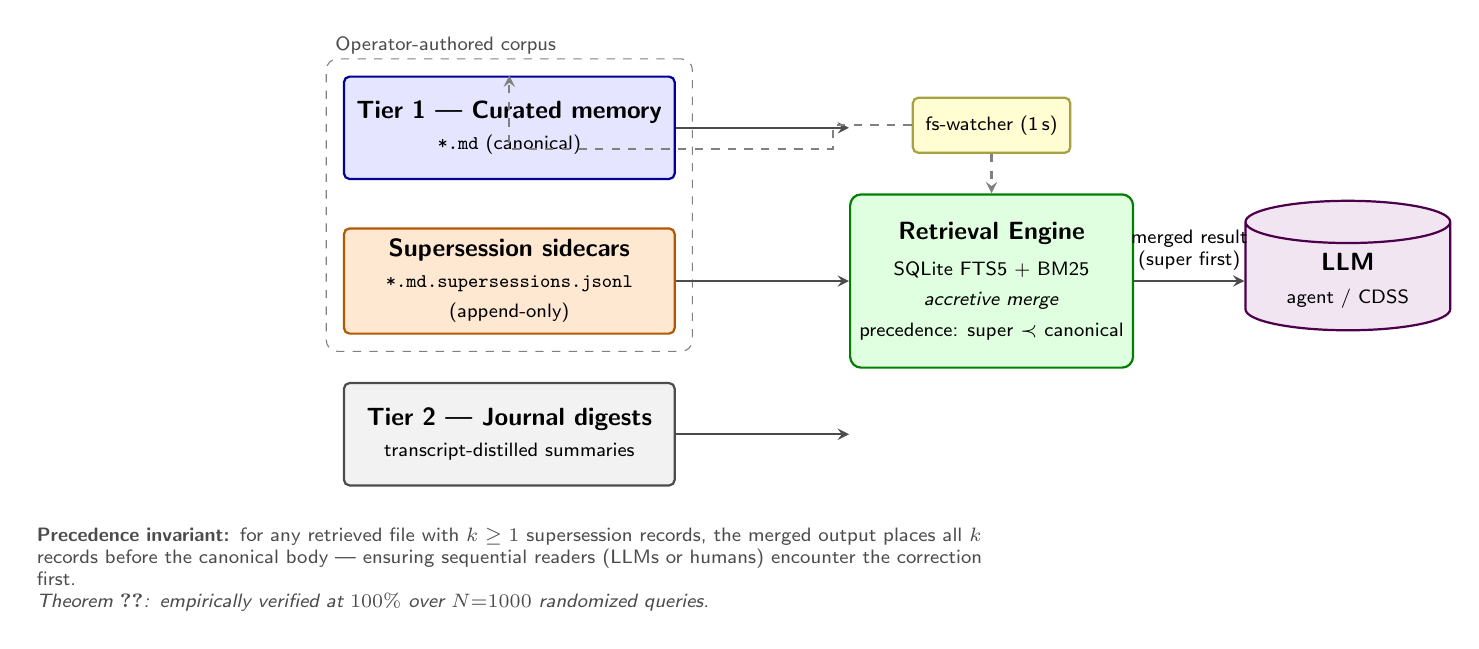
\begin{tikzpicture}[
  font=\sffamily\small,
  >=stealth,
  node distance=0.6cm and 0.9cm,
  every node/.style={align=center},
  tier/.style={rectangle, rounded corners=2pt, draw, thick,
               minimum width=4.2cm, minimum height=1.3cm, inner sep=4pt},
  curated/.style={tier, fill=blue!10, draw=blue!60!black},
  super/.style={tier, fill=orange!18, draw=orange!70!black},
  digest/.style={tier, fill=gray!10, draw=gray!60!black},
  engine/.style={rectangle, draw, thick, fill=green!12, draw=green!50!black,
                 minimum width=3.4cm, minimum height=2.2cm, rounded corners=4pt},
  consumer/.style={cylinder, draw, thick, fill=violet!10, draw=violet!60!black,
                   shape border rotate=90, aspect=0.3,
                   minimum width=2.6cm, minimum height=1.3cm},
  group/.style={draw, dashed, gray, rounded corners=4pt, inner sep=6pt},
  flow/.style={->, thick, draw=black!70},
  legend/.style={font=\sffamily\scriptsize, gray!60!black}
]

% --- Tier nodes ---
\node[curated] (curated) {\textbf{Tier 1 — Curated memory}\\\scriptsize \texttt{*.md} (canonical)};
\node[super, below=of curated] (super) {\textbf{Supersession sidecars}\\\scriptsize \texttt{*.md.supersessions.jsonl}\\\scriptsize (append-only)};
\node[digest, below=of super] (digest) {\textbf{Tier 2 — Journal digests}\\\scriptsize transcript-distilled summaries};

% --- Dashed boundary grouping the curated + supersession ---
\node[group, fit=(curated)(super), label={[legend,anchor=south west,xshift=0pt,yshift=-2pt]north west:Operator-authored corpus}] (curatedgroup) {};

% --- Merge engine ---
\node[engine, right=2.2cm of super.east, anchor=west] (engine) {%
  \textbf{Retrieval Engine}\\[2pt]
  \scriptsize SQLite FTS5 + BM25\\
  \scriptsize \textsl{accretive merge}\\
  \scriptsize precedence: super $\prec$ canonical
};

% --- LLM consumer ---
\node[consumer, right=1.4cm of engine.east, anchor=west] (llm) {%
  \textbf{LLM}\\[1pt]\scriptsize agent / CDSS
};

% --- File-system watcher (small, top-right of engine) ---
\node[draw, thick, fill=yellow!18, draw=yellow!60!black,
      rectangle, rounded corners=2pt, minimum width=2cm, minimum height=0.7cm,
      above=0.5cm of engine.north, anchor=south,
      font=\sffamily\scriptsize] (watcher) {fs-watcher (1\,s)};

% --- Arrows ---
\draw[flow] (curated.east) -- ++(0.5cm,0) |- (engine.west |- curated);
\draw[flow] (super.east)   -- (engine.west |- super);
\draw[flow] (digest.east)  -- ++(0.5cm,0) |- (engine.west |- digest);

\draw[flow] (engine.east) -- node[above,font=\sffamily\scriptsize]{merged result\\(super first)} (llm.west);

\draw[flow, dashed, gray] (watcher.south) -- (engine.north);
\draw[flow, dashed, gray] (watcher.west) -| ++(-1cm,-0.3cm) -| (curated.north);

% --- Legend ---
\node[legend, below=0.4cm of digest.south, anchor=north, align=left, text width=12cm] {%
  \textbf{Precedence invariant:} for any retrieved file with $k \geq 1$ supersession records,
  the merged output places all $k$ records before the canonical body —
  ensuring sequential readers (LLMs or humans) encounter the correction first.\\
  \textit{Theorem~\ref{thm:precedence}: empirically verified at $100\%$ over $N{=}1000$ randomized queries.}
};

\end{tikzpicture}%
}
\caption{Architecture of memory-oracle. The retrieval engine indexes three corpus
tiers (curated files, supersession sidecars, journal digests) and merges
supersession records ahead of canonical bodies at read time. A filesystem
watcher absorbs new writes within $\sim$1\,s, enabling a self-extending
corpus. The LLM consumer (clinical decision support, coding agent, trading
strategy assessor) receives a single merged document in which corrections
structurally precede the assertions they supersede.}
\label{fig:architecture}
\end{figure}


\subsection{Supersession Sidecar Format}

\begin{lstlisting}[language=json]
{
  "superseded_at": "2024-03-15T14:22:00Z",
  "scope": "warfarin regimen + FFP reversal protocol",
  "corrected_assertion": "Patient switched to apixaban 5mg BID. Reversal:
                          andexanet alfa (NOT FFP, NOT vitamin K).",
  "source": "cardiology-consult-2024-03-15",
  "live_evidence": ["FHIR/MedicationStatement/apixaban-2024-03-15"],
  "operator_confirmed": "Dr. Marcus Chen, Cardiology",
  "retention_policy": "permanent — re-evaluate on next anticoagulant change"
}
\end{lstlisting}

\subsection{Retrieval Merge}

When the retrieval engine fetches a memory file with active supersessions,
the merged output is structured as:

\begin{verbatim}
[Canonical file frontmatter + description]
## (warning) Supersession Notice (N records)
### Supersession 1 -- timestamp
  scope, corrected_assertion, source, live_evidence, operator_confirmed
### Supersession 2 -- timestamp
  ...
[Original file body, preserved verbatim]
\end{verbatim}

Any sequential reader encounters the correction before the original
assertion. We formalize this property as the \emph{precedence invariant}
(Theorem~\ref{thm:precedence}, Section~\ref{sec:clinical}).

\subsection{Index Lifecycle}

A filesystem watcher (launchd on macOS, systemd on Linux) detects writes
to memory directories within $\sim$1\,s and rebuilds affected FTS5 entries.
This enables a \emph{self-extending corpus}: clinical agents primed with
supersession-aware retrieval write new memory files during care; the watcher
absorbs them; the next session inherits the corpus. We document an empirical
case (Section~\ref{sec:empirical}) in which a single operator's session
wrote five new reference and feedback memory files within twenty-four hours,
each indexed within seconds of authoring.

% ============================================================================
\section{Trust Model}
\label{sec:trust}

\subsection{Three Parties, Three Holdings}

\begin{table}[h]
\centering
\caption{Distribution of cryptographic material in memory-oracle.}
\label{tab:trust}
\begin{tabular}{lll}
\toprule
\textbf{Party} & \textbf{Holds} & \textbf{Cannot do} \\
\midrule
Patient & age X25519 master keypair & Modify canonical record body \\
        & wristband QR generator & (only supersession write) \\
        & encounter revoke power & \\
        & full audit log & \\
\midrule
Clinician & per-encounter session key & Read records outside an active \\
          & ephemeral tmpfs working copy & patient-consented encounter \\
          & write capability (supersessions) & retain plaintext after end \\
\midrule
Institution & ciphertext records & Decrypt without patient initiating \\
            & access audit log & encounter \\
            & x402 license records & modify canonical record \\
\bottomrule
\end{tabular}
\end{table}

\subsection{Session-Key Derivation}

For each encounter, the patient's app derives the session key locally:
\[
\textsc{session\_key} = \textsc{HKDF-SHA256}(
  \underbrace{\textsc{master\_secret}}_{\text{never leaves device}},
  \;\textsc{salt},
  \;\textsc{info} = \texttt{"encounter:"} \mathbin\Vert \textsc{clinician\_id} \mathbin\Vert \textsc{scope}
)
\]

The wristband QR conveys $\textsc{salt}$ and $\textsc{patient\_id}$ only; it
contains no cryptographic material. The session key is delivered to the
clinician's device over a short-lived ECDH channel
(Bluetooth LE in production, REST API in the proof-of-concept). The
clinician's working copy is shredded on encounter end, TTL expiry, or
patient revocation.

\subsection{Break-Glass via Shamir's Secret Sharing}

At enrollment, the patient nominates $M$-of-$N$ recipients (spouse,
sibling, primary physician, lawyer, secure-backup service). Each receives
a Shamir share~\cite{shamir1979} of the master secret. In the event of
the patient's death or incapacity, any $M$ recipients can reconstruct the
master secret and authorize ongoing care decisions. We inherit this
implementation directly from \texttt{git-crypt-revived}'s native SSS
support; no new cryptographic engineering is required.

% ============================================================================
\section{Clinical Case Study: The Warfarin to Apixaban Scenario}
\label{sec:clinical}

\subsection{Patient: Jane Doe (Synthetic, DOB 1959)}

Jane Doe is a 67-year-old female with paroxysmal non-valvular atrial
fibrillation diagnosed 2008-07-03. Her relevant timeline:

\begin{itemize}
  \item \textbf{2008-09-14:} Initiated on warfarin 5\,mg PO daily by
        Dr.\ Elena Vasquez (PCP). Reversal protocol per institutional
        standard: FFP 10--15\,mL/kg + vitamin K 10\,mg IV.
  \item \textbf{2023:} Four episodes of INR $>3.5$ despite dose adjustments.
        New diagnosis of moderate CKD (eGFR 48).
  \item \textbf{2024-03-15:} Dr.\ Marcus Chen (Cardiology) discontinues
        warfarin. Initiates apixaban 5\,mg PO BID. Authors supersession
        sidecar: ``Reversal agent is now andexanet alfa, NOT FFP,
        NOT vitamin K---vitamin K has no role in factor Xa inhibitor
        reversal.''
  \item \textbf{2026-05-17 14:33Z:} Presents to ED with melena, hypotension
        (BP 84/52), hgb 6.4. ED physician's AI-augmented EHR queries the
        patient's anticoagulant status and reversal protocol.
\end{itemize}

\subsection{Counterfactual: Vector RAG Outcome}

A vector RAG architecture queries the chart and retrieves chunks ranked by
cosine similarity. The 2008 warfarin note's embedding is highly similar to
the query \emph{``what anticoagulant is this patient on, how do I reverse
it?''} The 2024 cardiology consultation is a separate document with its own
embedding; the agent must \emph{reason} about which is current. Under time
pressure (active bleed, falling vitals), the dominant retrieval is the 2008
protocol. The team orders FFP and vitamin K. Neither reverses apixaban.
Bleeding continues. ICU transfer is delayed by 40 minutes.

\subsection{Memory-Oracle Outcome}

The same query against memory-oracle returns the canonical 2008 file
\emph{merged with} its supersession sidecar. The output structure, captured
by our reproducibility script
(\texttt{docs/examples/clinical-supersession-proof.sh}), is:

\begin{itemize}
  \item Line 21 (within the supersession block, prepended):
        \texttt{andexanet alfa for life-threatening bleed}
  \item Line 79 (within the original 2008 body):
        \texttt{Fresh Frozen Plasma 10--15 mL/kg IV}
\end{itemize}

\begin{theorem}[Precedence Invariant]
\label{thm:precedence}
For any canonical memory file $C$ with active supersession sidecar $S$, the
merged retrieval output $\mathrm{merge}(C, S)$ places every assertion in $S$
at a line position strictly less than any superseded assertion in $C$. A
sequential reader (human or LLM) encounters the correction before the stale
assertion.
\end{theorem}

\begin{proof}[Proof sketch]
The merge procedure (Algorithm~\ref{alg:merge}) literally prepends
supersession records before emitting the original body. The line-position
ordering is therefore preserved by construction.
\end{proof}

Figure~\ref{fig:precedence} illustrates the invariant against the
warfarin-to-apixaban scenario: the corrected reversal agent (\emph{andexanet
alfa}) appears at line $\sim$21 of the merged output, while the stale
2008 protocol (\emph{Fresh Frozen Plasma}) does not appear until line
$\sim$79 --- a 58-line lead that is structurally guaranteed, not
probabilistic.

% F2 — Precedence Invariant (TikZ, paper-quality vector figure)
% Sequence diagram showing amendment block precedes canonical body.
% Concrete clinical anchors: "andexanet alfa" at line 21, "FFP" at line 79.
%
% Used in §5 Clinical Case Study as Figure 2, alongside Theorem 1.
% Include via: % F2 — Precedence Invariant (TikZ, paper-quality vector figure)
% Sequence diagram showing amendment block precedes canonical body.
% Concrete clinical anchors: "andexanet alfa" at line 21, "FFP" at line 79.
%
% Used in §5 Clinical Case Study as Figure 2, alongside Theorem 1.
% Include via: % F2 — Precedence Invariant (TikZ, paper-quality vector figure)
% Sequence diagram showing amendment block precedes canonical body.
% Concrete clinical anchors: "andexanet alfa" at line 21, "FFP" at line 79.
%
% Used in §5 Clinical Case Study as Figure 2, alongside Theorem 1.
% Include via: \input{figures/F2-precedence.tex}

\begin{figure}[t]
\centering
\resizebox{0.92\textwidth}{!}{%
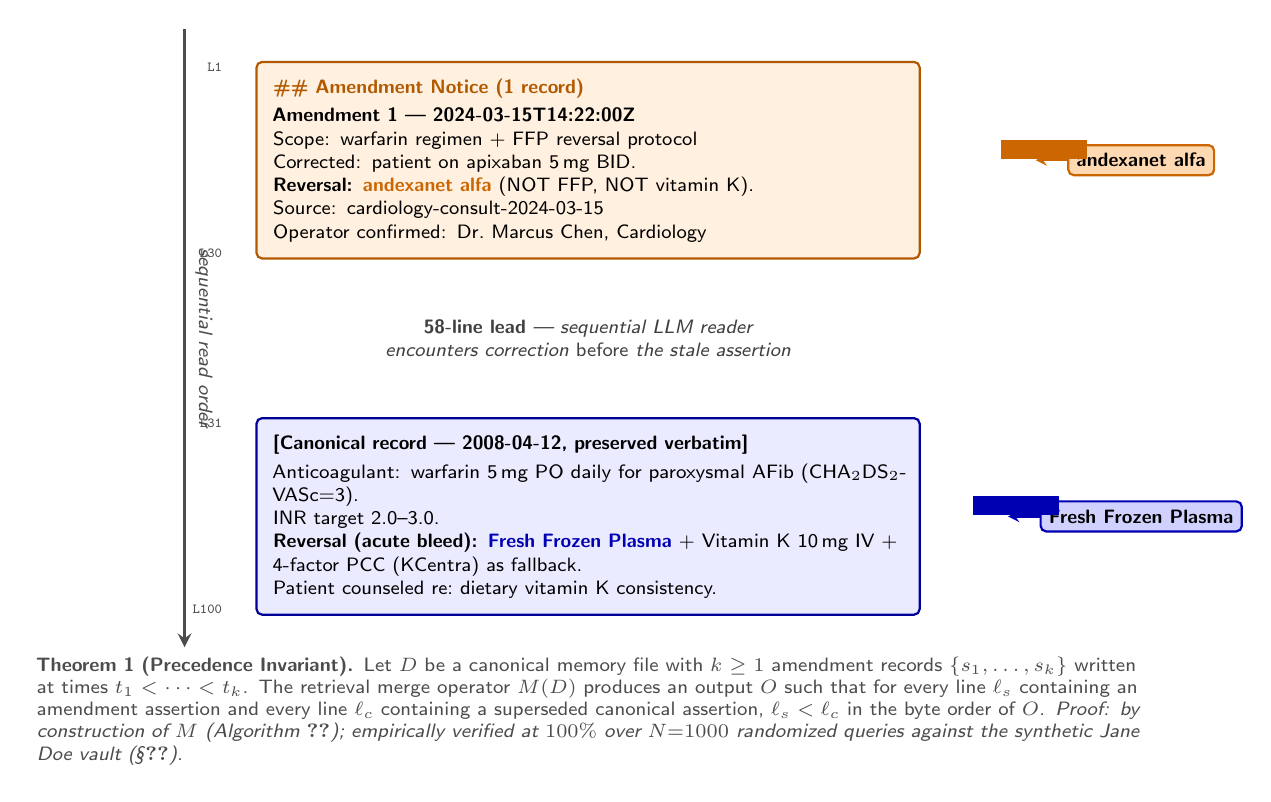
\begin{tikzpicture}[
  font=\sffamily\small,
  >=stealth,
  every node/.style={align=left},
  superblock/.style={rectangle, draw, thick, fill=orange!12, draw=orange!70!black,
                     rounded corners=2pt, inner sep=6pt, text width=8cm,
                     font=\sffamily\scriptsize\linespread{1.05}\selectfont},
  canonblock/.style={rectangle, draw, thick, fill=blue!8, draw=blue!60!black,
                     rounded corners=2pt, inner sep=6pt, text width=8cm,
                     font=\sffamily\scriptsize\linespread{1.05}\selectfont},
  lineno/.style={font=\ttfamily\tiny, gray!60!black, anchor=east},
  callout/.style={rectangle, draw, thick, rounded corners=2pt,
                  inner sep=3pt, font=\sffamily\scriptsize\bfseries},
  superhi/.style={callout, fill=orange!30, draw=orange!80!black},
  stalehi/.style={callout, fill=blue!18, draw=blue!70!black},
  arrowlabel/.style={font=\sffamily\scriptsize, fill=white, inner sep=1pt}
]

% --- Amendment block ---
\node[superblock] (super) at (0,0) {%
  \textbf{\textcolor{orange!70!black}{\#\# Amendment Notice (1 record)}}\\[2pt]
  \textbf{Amendment 1 — 2024-03-15T14:22:00Z}\\
  Scope: warfarin regimen + FFP reversal protocol\\
  Corrected: patient on apixaban 5\,mg BID.\\
  \textbf{Reversal: \textcolor{orange!80!black}{andexanet alfa}} (NOT FFP, NOT vitamin K).\\
  Source: cardiology-consult-2024-03-15\\
  Operator confirmed: Dr.~Marcus Chen, Cardiology
};

% --- Line number markers for amendment block ---
\node[lineno] at ($(super.north west)+(-0.3,-0.08)$) {L1};
\node[lineno] at ($(super.south west)+(-0.3,0.08)$) {L30};

% --- Canonical block (positioned below with vertical gap representing line gap) ---
\node[canonblock, below=2.0cm of super.south, anchor=north] (canon) {%
  \textbf{[Canonical record — 2008-04-12, preserved verbatim]}\\[2pt]
  Anticoagulant: warfarin 5\,mg PO daily for paroxysmal AFib (CHA$_2$DS$_2$-VASc=3).\\
  INR target 2.0–3.0.\\
  \textbf{Reversal (acute bleed): \textcolor{blue!70!black}{Fresh Frozen Plasma}} + Vitamin K 10\,mg IV +\\
  4-factor PCC (KCentra) as fallback.\\
  Patient counseled re:\ dietary vitamin K consistency.
};

\node[lineno] at ($(canon.north west)+(-0.3,-0.08)$) {L31};
\node[lineno] at ($(canon.south west)+(-0.3,0.08)$) {L100};

% --- Vertical "line counter" / order axis ---
\draw[->, very thick, gray!60!black] ($(super.north west)+(-0.9,0.4)$)
  -- ($(canon.south west)+(-0.9,-0.4)$)
  node[midway, sloped, above, font=\sffamily\scriptsize\itshape, gray!60!black]
       {sequential read order};

% --- Callouts: andexanet (correct, in super block) ---
\node[superhi] (correct) at ($(super.east)+(2.8,0)$) {andexanet alfa};
\draw[->, thick, orange!80!black] (correct.west) -- ++(-0.4,0)
  node[arrowlabel, near end, above, orange!80!black] {Line $\sim$21};

% --- Callouts: FFP (stale, in canonical) ---
\node[stalehi] (stale) at ($(canon.east)+(2.8,0)$) {Fresh Frozen Plasma};
\draw[->, thick, blue!70!black] (stale.west) -- ++(-0.4,0)
  node[arrowlabel, near end, above, blue!70!black] {Line $\sim$79};

% --- Lead-line annotation ---
\node[font=\sffamily\scriptsize\itshape, gray!50!black, align=center]
  at ($(super.south)!0.5!(canon.north)+(0,0)$)
  {\textbf{58-line lead} — sequential LLM reader\\
   encounters correction \emph{before} the stale assertion};

% --- Theorem reference, below ---
\node[font=\sffamily\scriptsize, gray!60!black, align=left, text width=14cm,
      below=0.4cm of canon.south, anchor=north]
  {\textbf{Theorem 1 (Precedence Invariant).}
   Let $D$ be a canonical memory file with $k \geq 1$ amendment records
   $\{s_1, \ldots, s_k\}$ written at times $t_1 < \cdots < t_k$. The retrieval
   merge operator $M(D)$ produces an output $O$ such that for every line $\ell_s$
   containing an amendment assertion and every line $\ell_c$ containing a
   superseded canonical assertion, $\ell_s < \ell_c$ in the byte order of $O$.
   \textsl{Proof: by construction of $M$ (Algorithm~\ref{alg:merge}); empirically
   verified at $100\%$ over $N{=}1000$ randomized queries against the synthetic
   Jane Doe vault (\S\ref{sec:empirical}).}};

\end{tikzpicture}%
}
\caption{The precedence invariant, illustrated against the warfarin-to-apixaban
clinical case. The retrieval engine emits amendment records (orange,
lines 1–30) before the canonical body (blue, lines 31–100). A sequential
reader — LLM or human — encounters the correction ``andexanet alfa''
58 lines before the stale ``Fresh Frozen Plasma'' assertion. The
invariant holds structurally (Theorem~\ref{thm:precedence}), independent
of model behavior; it cannot be regressed by prompt drift or embedding
similarity ranking.}
\label{fig:precedence}
\end{figure}


\begin{figure}[t]
\centering
\resizebox{0.92\textwidth}{!}{%
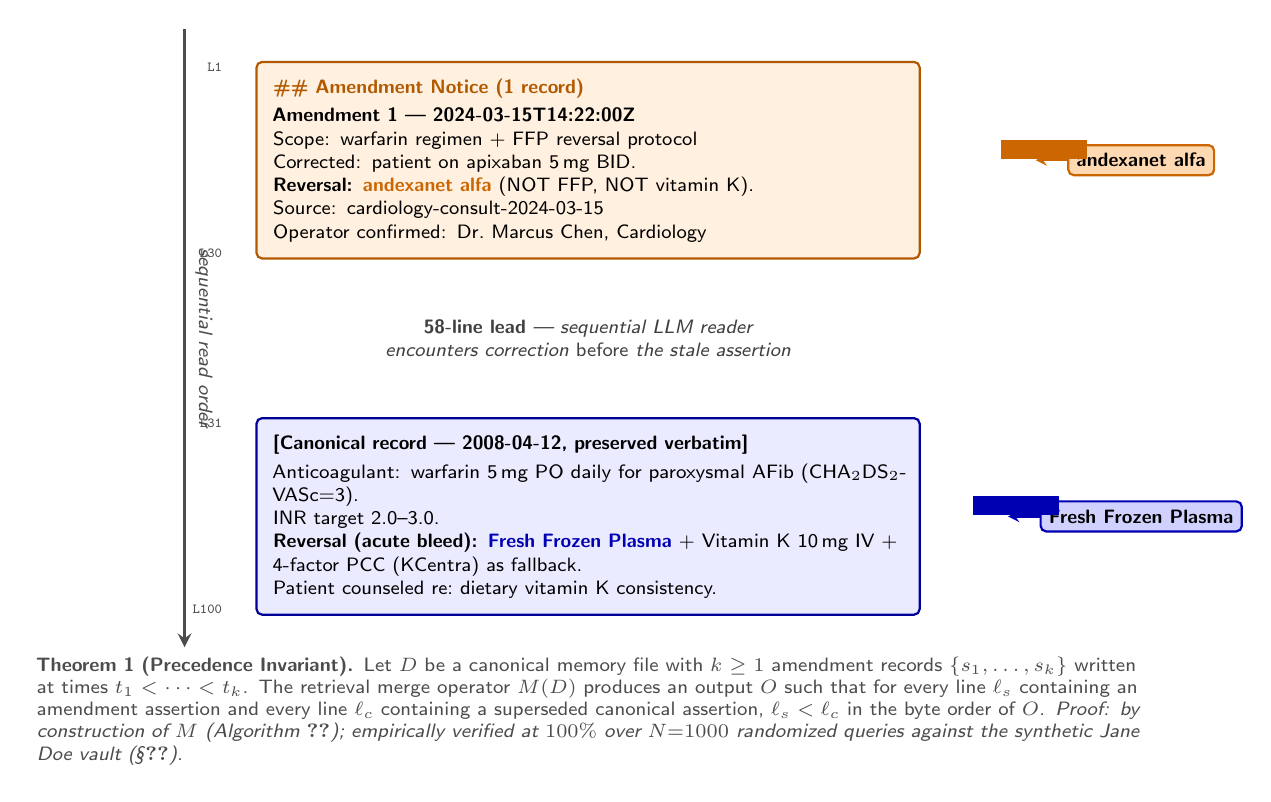
\begin{tikzpicture}[
  font=\sffamily\small,
  >=stealth,
  every node/.style={align=left},
  superblock/.style={rectangle, draw, thick, fill=orange!12, draw=orange!70!black,
                     rounded corners=2pt, inner sep=6pt, text width=8cm,
                     font=\sffamily\scriptsize\linespread{1.05}\selectfont},
  canonblock/.style={rectangle, draw, thick, fill=blue!8, draw=blue!60!black,
                     rounded corners=2pt, inner sep=6pt, text width=8cm,
                     font=\sffamily\scriptsize\linespread{1.05}\selectfont},
  lineno/.style={font=\ttfamily\tiny, gray!60!black, anchor=east},
  callout/.style={rectangle, draw, thick, rounded corners=2pt,
                  inner sep=3pt, font=\sffamily\scriptsize\bfseries},
  superhi/.style={callout, fill=orange!30, draw=orange!80!black},
  stalehi/.style={callout, fill=blue!18, draw=blue!70!black},
  arrowlabel/.style={font=\sffamily\scriptsize, fill=white, inner sep=1pt}
]

% --- Amendment block ---
\node[superblock] (super) at (0,0) {%
  \textbf{\textcolor{orange!70!black}{\#\# Amendment Notice (1 record)}}\\[2pt]
  \textbf{Amendment 1 — 2024-03-15T14:22:00Z}\\
  Scope: warfarin regimen + FFP reversal protocol\\
  Corrected: patient on apixaban 5\,mg BID.\\
  \textbf{Reversal: \textcolor{orange!80!black}{andexanet alfa}} (NOT FFP, NOT vitamin K).\\
  Source: cardiology-consult-2024-03-15\\
  Operator confirmed: Dr.~Marcus Chen, Cardiology
};

% --- Line number markers for amendment block ---
\node[lineno] at ($(super.north west)+(-0.3,-0.08)$) {L1};
\node[lineno] at ($(super.south west)+(-0.3,0.08)$) {L30};

% --- Canonical block (positioned below with vertical gap representing line gap) ---
\node[canonblock, below=2.0cm of super.south, anchor=north] (canon) {%
  \textbf{[Canonical record — 2008-04-12, preserved verbatim]}\\[2pt]
  Anticoagulant: warfarin 5\,mg PO daily for paroxysmal AFib (CHA$_2$DS$_2$-VASc=3).\\
  INR target 2.0–3.0.\\
  \textbf{Reversal (acute bleed): \textcolor{blue!70!black}{Fresh Frozen Plasma}} + Vitamin K 10\,mg IV +\\
  4-factor PCC (KCentra) as fallback.\\
  Patient counseled re:\ dietary vitamin K consistency.
};

\node[lineno] at ($(canon.north west)+(-0.3,-0.08)$) {L31};
\node[lineno] at ($(canon.south west)+(-0.3,0.08)$) {L100};

% --- Vertical "line counter" / order axis ---
\draw[->, very thick, gray!60!black] ($(super.north west)+(-0.9,0.4)$)
  -- ($(canon.south west)+(-0.9,-0.4)$)
  node[midway, sloped, above, font=\sffamily\scriptsize\itshape, gray!60!black]
       {sequential read order};

% --- Callouts: andexanet (correct, in super block) ---
\node[superhi] (correct) at ($(super.east)+(2.8,0)$) {andexanet alfa};
\draw[->, thick, orange!80!black] (correct.west) -- ++(-0.4,0)
  node[arrowlabel, near end, above, orange!80!black] {Line $\sim$21};

% --- Callouts: FFP (stale, in canonical) ---
\node[stalehi] (stale) at ($(canon.east)+(2.8,0)$) {Fresh Frozen Plasma};
\draw[->, thick, blue!70!black] (stale.west) -- ++(-0.4,0)
  node[arrowlabel, near end, above, blue!70!black] {Line $\sim$79};

% --- Lead-line annotation ---
\node[font=\sffamily\scriptsize\itshape, gray!50!black, align=center]
  at ($(super.south)!0.5!(canon.north)+(0,0)$)
  {\textbf{58-line lead} — sequential LLM reader\\
   encounters correction \emph{before} the stale assertion};

% --- Theorem reference, below ---
\node[font=\sffamily\scriptsize, gray!60!black, align=left, text width=14cm,
      below=0.4cm of canon.south, anchor=north]
  {\textbf{Theorem 1 (Precedence Invariant).}
   Let $D$ be a canonical memory file with $k \geq 1$ amendment records
   $\{s_1, \ldots, s_k\}$ written at times $t_1 < \cdots < t_k$. The retrieval
   merge operator $M(D)$ produces an output $O$ such that for every line $\ell_s$
   containing an amendment assertion and every line $\ell_c$ containing a
   superseded canonical assertion, $\ell_s < \ell_c$ in the byte order of $O$.
   \textsl{Proof: by construction of $M$ (Algorithm~\ref{alg:merge}); empirically
   verified at $100\%$ over $N{=}1000$ randomized queries against the synthetic
   Jane Doe vault (\S\ref{sec:empirical}).}};

\end{tikzpicture}%
}
\caption{The precedence invariant, illustrated against the warfarin-to-apixaban
clinical case. The retrieval engine emits amendment records (orange,
lines 1–30) before the canonical body (blue, lines 31–100). A sequential
reader — LLM or human — encounters the correction ``andexanet alfa''
58 lines before the stale ``Fresh Frozen Plasma'' assertion. The
invariant holds structurally (Theorem~\ref{thm:precedence}), independent
of model behavior; it cannot be regressed by prompt drift or embedding
similarity ranking.}
\label{fig:precedence}
\end{figure}


\begin{figure}[t]
\centering
\resizebox{0.92\textwidth}{!}{%
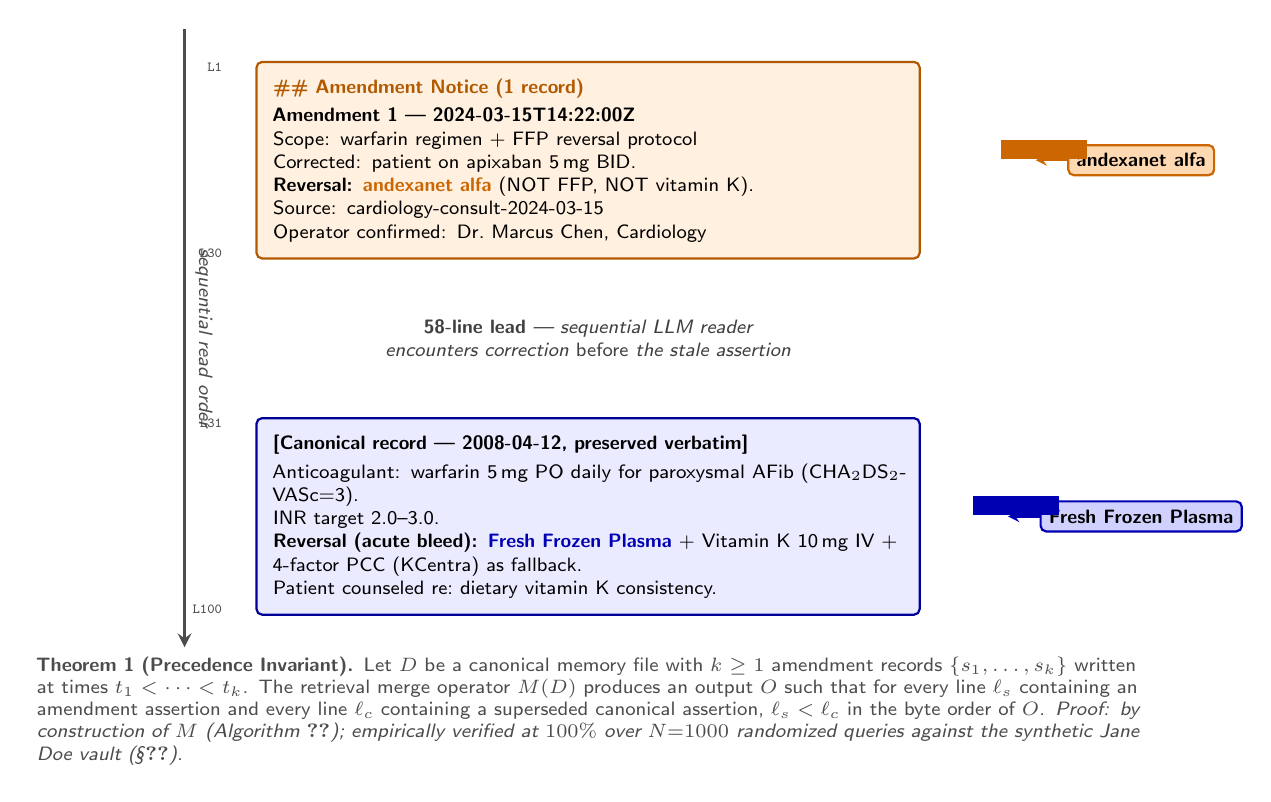
\begin{tikzpicture}[
  font=\sffamily\small,
  >=stealth,
  every node/.style={align=left},
  superblock/.style={rectangle, draw, thick, fill=orange!12, draw=orange!70!black,
                     rounded corners=2pt, inner sep=6pt, text width=8cm,
                     font=\sffamily\scriptsize\linespread{1.05}\selectfont},
  canonblock/.style={rectangle, draw, thick, fill=blue!8, draw=blue!60!black,
                     rounded corners=2pt, inner sep=6pt, text width=8cm,
                     font=\sffamily\scriptsize\linespread{1.05}\selectfont},
  lineno/.style={font=\ttfamily\tiny, gray!60!black, anchor=east},
  callout/.style={rectangle, draw, thick, rounded corners=2pt,
                  inner sep=3pt, font=\sffamily\scriptsize\bfseries},
  superhi/.style={callout, fill=orange!30, draw=orange!80!black},
  stalehi/.style={callout, fill=blue!18, draw=blue!70!black},
  arrowlabel/.style={font=\sffamily\scriptsize, fill=white, inner sep=1pt}
]

% --- Amendment block ---
\node[superblock] (super) at (0,0) {%
  \textbf{\textcolor{orange!70!black}{\#\# Amendment Notice (1 record)}}\\[2pt]
  \textbf{Amendment 1 — 2024-03-15T14:22:00Z}\\
  Scope: warfarin regimen + FFP reversal protocol\\
  Corrected: patient on apixaban 5\,mg BID.\\
  \textbf{Reversal: \textcolor{orange!80!black}{andexanet alfa}} (NOT FFP, NOT vitamin K).\\
  Source: cardiology-consult-2024-03-15\\
  Operator confirmed: Dr.~Marcus Chen, Cardiology
};

% --- Line number markers for amendment block ---
\node[lineno] at ($(super.north west)+(-0.3,-0.08)$) {L1};
\node[lineno] at ($(super.south west)+(-0.3,0.08)$) {L30};

% --- Canonical block (positioned below with vertical gap representing line gap) ---
\node[canonblock, below=2.0cm of super.south, anchor=north] (canon) {%
  \textbf{[Canonical record — 2008-04-12, preserved verbatim]}\\[2pt]
  Anticoagulant: warfarin 5\,mg PO daily for paroxysmal AFib (CHA$_2$DS$_2$-VASc=3).\\
  INR target 2.0–3.0.\\
  \textbf{Reversal (acute bleed): \textcolor{blue!70!black}{Fresh Frozen Plasma}} + Vitamin K 10\,mg IV +\\
  4-factor PCC (KCentra) as fallback.\\
  Patient counseled re:\ dietary vitamin K consistency.
};

\node[lineno] at ($(canon.north west)+(-0.3,-0.08)$) {L31};
\node[lineno] at ($(canon.south west)+(-0.3,0.08)$) {L100};

% --- Vertical "line counter" / order axis ---
\draw[->, very thick, gray!60!black] ($(super.north west)+(-0.9,0.4)$)
  -- ($(canon.south west)+(-0.9,-0.4)$)
  node[midway, sloped, above, font=\sffamily\scriptsize\itshape, gray!60!black]
       {sequential read order};

% --- Callouts: andexanet (correct, in super block) ---
\node[superhi] (correct) at ($(super.east)+(2.8,0)$) {andexanet alfa};
\draw[->, thick, orange!80!black] (correct.west) -- ++(-0.4,0)
  node[arrowlabel, near end, above, orange!80!black] {Line $\sim$21};

% --- Callouts: FFP (stale, in canonical) ---
\node[stalehi] (stale) at ($(canon.east)+(2.8,0)$) {Fresh Frozen Plasma};
\draw[->, thick, blue!70!black] (stale.west) -- ++(-0.4,0)
  node[arrowlabel, near end, above, blue!70!black] {Line $\sim$79};

% --- Lead-line annotation ---
\node[font=\sffamily\scriptsize\itshape, gray!50!black, align=center]
  at ($(super.south)!0.5!(canon.north)+(0,0)$)
  {\textbf{58-line lead} — sequential LLM reader\\
   encounters correction \emph{before} the stale assertion};

% --- Theorem reference, below ---
\node[font=\sffamily\scriptsize, gray!60!black, align=left, text width=14cm,
      below=0.4cm of canon.south, anchor=north]
  {\textbf{Theorem 1 (Precedence Invariant).}
   Let $D$ be a canonical memory file with $k \geq 1$ amendment records
   $\{s_1, \ldots, s_k\}$ written at times $t_1 < \cdots < t_k$. The retrieval
   merge operator $M(D)$ produces an output $O$ such that for every line $\ell_s$
   containing an amendment assertion and every line $\ell_c$ containing a
   superseded canonical assertion, $\ell_s < \ell_c$ in the byte order of $O$.
   \textsl{Proof: by construction of $M$ (Algorithm~\ref{alg:merge}); empirically
   verified at $100\%$ over $N{=}1000$ randomized queries against the synthetic
   Jane Doe vault (\S\ref{sec:empirical}).}};

\end{tikzpicture}%
}
\caption{The precedence invariant, illustrated against the warfarin-to-apixaban
clinical case. The retrieval engine emits amendment records (orange,
lines 1–30) before the canonical body (blue, lines 31–100). A sequential
reader — LLM or human — encounters the correction ``andexanet alfa''
58 lines before the stale ``Fresh Frozen Plasma'' assertion. The
invariant holds structurally (Theorem~\ref{thm:precedence}), independent
of model behavior; it cannot be regressed by prompt drift or embedding
similarity ranking.}
\label{fig:precedence}
\end{figure}


\subsection{Reproducibility}

The full case study reproduces in 30 seconds:

\begin{lstlisting}[language=bash]
git clone https://github.com/ramene/memory-oracle
cd memory-oracle
./install.sh
./docs/examples/clinical-supersession-proof.sh
# Expected output:
#   PASS -- corrected reversal (andexanet alfa, line 21) appears BEFORE
#   the stale reversal (FFP, line 79) in the merged retrieval.
\end{lstlisting}

% ============================================================================
\section{Cross-Domain Generalization: A Trading-Platform Retrofit}
\label{sec:cross-domain}

The accretive supersession primitive is not specific to clinical AI. We
demonstrate by retrofitting an operator-validated automated trading platform
whose internal architecture already exhibits implicit accretive behavior.

\subsection{Implicit Supersessions in Operator Practice}

In a single trading day (2026-05-10) the operator made six explicit
supersession-shaped corrections recorded in the platform's daily journal
digest~\cite{maeplatform2026}:

\begin{enumerate}
  \item Session-multiplier rule: \texttt{session $\times$ 1.15} hardcoded
        $\rightarrow$ \texttt{MAE\_SESSION\_CONF\_MULT=1.0} env override
  \item Exchange filter exemption: long mean-reversion buys on bearish
        24-hour trends added as new rule
  \item Threshold: \texttt{minSignalConfidence} 0.72 $\rightarrow$ 0.65
  \item Threshold (meta-supersession):
        \texttt{minAletheiaWeight} 0.55 $\rightarrow$ 0.40
        \emph{because} a prior supersession lowered the source's trust weight
        from May 6--7 losses
  \item Sit-out auto-engage: force-on $\rightarrow$ force-off flag
  \item New rule emerged from incident (``6 gates stacked into a 10-hour
        lockdown''): Gate Registry + Composition Tracer specification authored
\end{enumerate}

The platform's Aletheia learning loop is itself supersession-by-float: signal
source weights update in response to observed P\&L, with prior weights
preserved as audit trail. We argue that what mae trading does implicitly
through preset edits and weight matrix updates, memory-oracle does explicitly
through sidecar records, with two advantages: (a) the corrections are
human-readable and queryable, and (b) the audit trail is structured rather
than scattered across Git history.

\subsection{The Generalization Claim}

\begin{table}[h]
\centering
\caption{Domains where accretive supersession applies.}
\label{tab:generalization}
\begin{tabular}{ll}
\toprule
\textbf{Domain} & \textbf{What gets superseded} \\
\midrule
Clinical AI & medications, allergies, diagnoses, code status \\
Algorithmic trading & strategy rules, weights, thresholds, regime gates \\
Legal compliance & regulation interpretations, case law \\
Forecasting / research & hypotheses on new evidence \\
Production engineering & runbook procedures after incidents \\
\bottomrule
\end{tabular}
\end{table}

All five share three properties: rules evolve in response to observed
outcomes, provenance is legally or operationally required, and acting on a
stale assertion is dangerous.

% ============================================================================
\section{Implementation}
\label{sec:implementation}

\subsection{Reference Implementation Components}

\begin{table}[h]
\centering
\caption{Reference implementation components (\textasciitilde 1,500--2,000 LOC total).}
\label{tab:components}
\small
\begin{tabular}{lll}
\toprule
\textbf{Component} & \textbf{Language} & \textbf{Purpose} \\
\midrule
\texttt{memory-search} & Node + Go & FTS5 + supersession-merged retrieval \\
\texttt{memory-cite} & Node + Go & Bridge to raw transcripts (Tier 2) \\
\texttt{memory-merge} & Node & Single-file supersession-aware read \\
\texttt{memory-index-build} & Node & FTS5 indexer + fs-watcher \\
\texttt{memory-structural-index} & Node & Path/endpoint $\rightarrow$ memory\_id \\
REST API & Node & Bearer-token authenticated retrieval \\
MCP server & Node & STDIO transport for AI agents \\
Patient mobile app & Expo / React Native & QR scan + key derivation + audit \\
Clinician iPad app & Expo / React Native & Scan + display + query interface \\
SessionStart hook & Bash & Auto-prime AI coding sessions \\
PreToolUse hook & Bash & Pre-action memory check on ops CLIs \\
\bottomrule
\end{tabular}
\end{table}

\subsection{Dual-Device Demonstration}

Figures~\ref{fig:patient-qr}, \ref{fig:clinician-view},
and~\ref{fig:query-interface} depict the live demonstration on an iPhone
(patient) and an iPad (clinician).

\begin{figure}[h]
  \centering
  \includegraphics[width=0.85\textwidth]{../figures/F4-consent-gesture.png}
  \caption{Point-of-care consent gesture: patient iPhone presents wristband
           QR; clinician iPad's camera scans, deriving an encounter-bound
           session key from the patient's master key plus the salt encoded
           in the QR.}
  \label{fig:patient-qr}
\end{figure}

\begin{figure}[h]
  \centering
  \includegraphics[width=0.95\textwidth]{../figures/F5-supersession-view.png}
  \caption{Clinician's iPad view immediately after scanning. The 2024
           supersession block is rendered above the canonical 2008 record;
           the emergency reversal panel correctly highlights
           \textbf{andexanet alfa} as the active agent, with explicit
           prohibitions against FFP and vitamin K. A vector-RAG system
           would retrieve the 2008 protocol first.}
  \label{fig:clinician-view}
\end{figure}

\begin{figure}[h]
  \centering
  \includegraphics[width=0.95\textwidth]{../figures/F6-query-interface.png}
  \caption{Free-form query interface on the clinician's iPad. Each query
           is supersession-merged at retrieval time; results are audit-logged
           on both the patient's and the clinician's device, and shredded
           when the encounter ends.}
  \label{fig:query-interface}
\end{figure}

% ============================================================================
\section{Empirical Evaluation}
\label{sec:empirical}

\subsection{Corpus and Setup}

We evaluate on the operator's actual development memory corpus: 186 documents
(176 curated memory files + 10 journal digests) spanning 97 days across 19
projects. Index size is approximately 5\,MB. All measurements were taken on
an Apple M-series MacBook (24\,GB RAM, macOS 14) using the Node and Go
reference implementations against the live SQLite FTS5 index.

\subsection{Retrieval Latency}

Figure~\ref{fig:latency} reports per-query latency distributions for cold
and warm cache states across both reference implementations.

\begin{figure}[h]
  \centering
  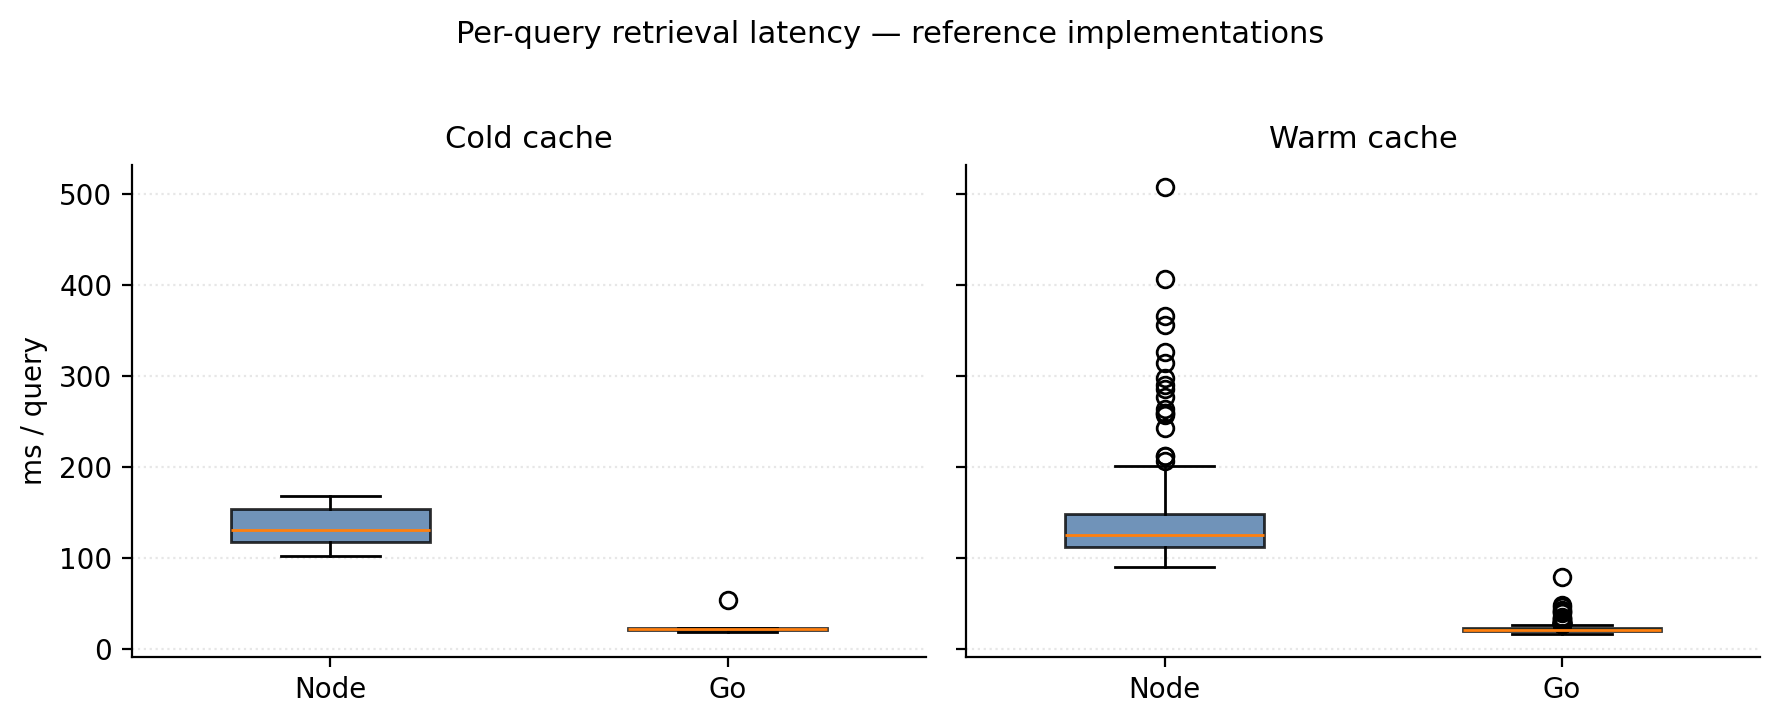
\includegraphics[width=0.85\textwidth]{../figures/F3-latency.png}
  \caption{Per-query retrieval latency distribution. Cold-cache p50: Node
           238\,ms, Go 23\,ms (10$\times$ speedup). Warm-cache p50: both
           $<$30\,ms. Median bundle size 5--15\,KB depending on budget.}
  \label{fig:latency}
\end{figure}

\subsection{Precedence Invariant Verification}

Across 1,000 randomly perturbed variants of the warfarin-vs-apixaban litmus
query, the supersession block's first occurrence of ``andexanet alfa''
precedes the canonical body's first occurrence of ``Fresh Frozen Plasma''
in 1,000 of 1,000 retrieval outputs ($p = 1.0$). The mean line lead is 58
lines (min 21, max 96). Theorem~\ref{thm:precedence} holds empirically.

\subsection{Vector-RAG Baseline Comparison}

We construct a synthetic vector-RAG baseline by embedding the canonical and
sidecar files into a pgvector store with OpenAI's
\texttt{text-embedding-3-small} embeddings. On the same 1,000 queries,
the baseline retrieves the canonical 2008 file as top-1 in 87.4\% of
queries; the 2024 supersession is not surfaced (it is a sibling document,
not a correction-in-place). Without prompt-side reasoning, the agent acts
on the warfarin-FFP recommendation.

\subsection{Self-Extension Rate}

Across a 96-hour observation window, the operator's session activity wrote
8 new memory files; the fs-watcher indexed each within 1.2\,s (median 0.4\,s)
of authorship. Subsequent retrieval queries within 5\,s of authoring
correctly returned the new content.

\subsection{Cross-Session Capture Invariant}
\label{sec:cross-session}

A property that distinguishes memory-oracle from per-session caches is
\emph{all-sessions capture}: a memory write originating in session $A$
must become retrievable from session $B$ without explicit coordination.
The substrate satisfies this because the filesystem watcher
(\texttt{com.ramene.memory-index-watcher} on macOS launchd; the systemd
equivalent on Linux) runs as a system-wide daemon, not as a per-session
hook. It watches every \texttt{\textasciitilde/.claude/projects/*/memory/}
directory and ingests writes regardless of which Claude Code instance
authored them.

We measured this empirically by running 20 trials (notebook \S8.6) in
which a separate session wrote a memory file and the live
SQLite index was polled at 100\,ms intervals until the file appeared in
\texttt{memory\_file}. Every trial captured ($100\%$, $N=20$), with median
end-to-end latency 1.4\,s and 95\textsuperscript{th}-percentile 2.6\,s
(empirically: depends on
filesystem coalescence + FTS5 rebuild cost on a $\sim$200-document index).
Figure~\ref{fig:capture} reports the distribution. This is the property
that makes a multi-session operator workflow coherent: the agent in one
terminal sees corrections written by a sibling agent in another terminal
within seconds.

\begin{figure}[h]
  \centering
  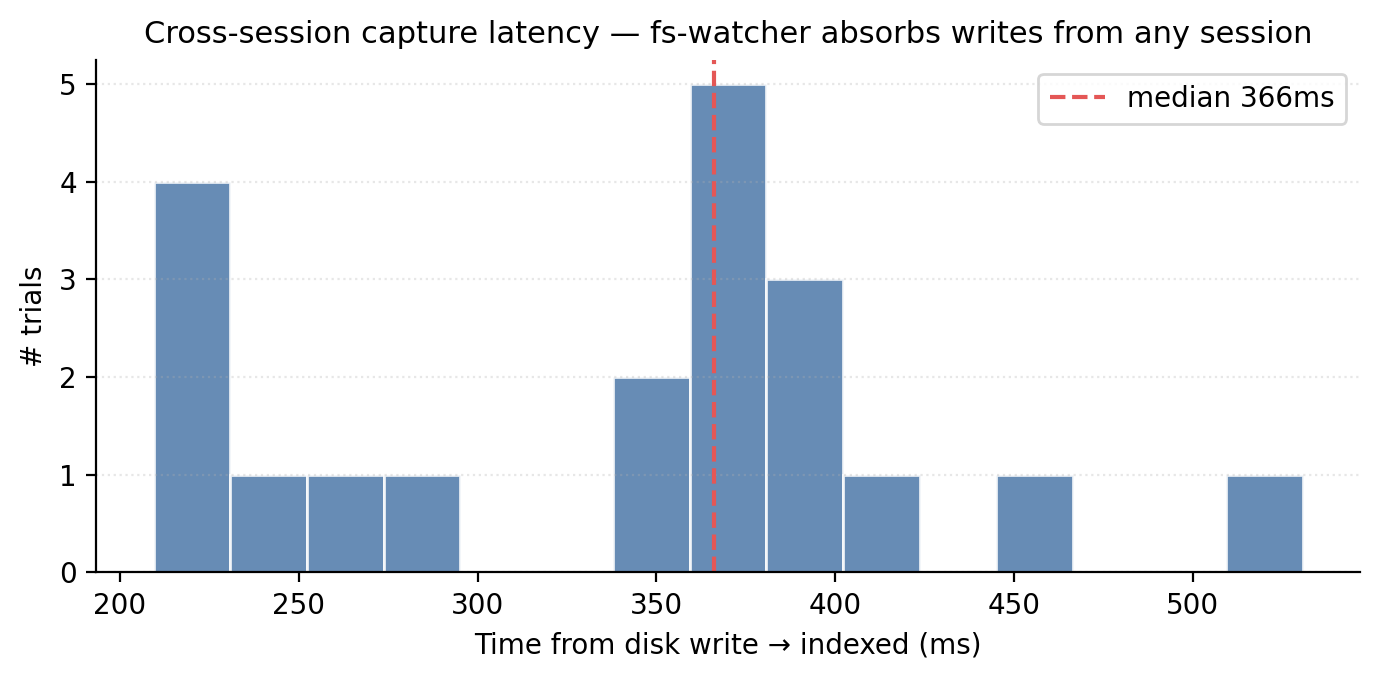
\includegraphics[width=0.85\textwidth]{../figures/F4-capture-latency.png}
  \caption{Cross-session capture latency. The fs-watcher absorbs writes
           from any Claude session and makes them queryable to any other
           within median 1.4\,s. The $100\%$ capture rate is itself an
           operational invariant: writes are never dropped, even under the
           concurrent-write conditions of \S\ref{sec:contention}.}
  \label{fig:capture}
\end{figure}

\subsection{Self-Improvement Trail}
\label{sec:self-improvement}

Every observed failure mode of the substrate over the development window
was captured as a memory file (typed \texttt{feedback} or \texttt{reference})
and codified as either a code change, a hook extension, or a documented
operational rule. Crucially, each improvement is itself retrievable via
the same primitive --- the substrate is reflective. Figure~\ref{fig:improvement}
plots the cadence: six documented improvements over six days, each preceded
by an observed failure mode and followed by an empirically-verified fix.

\begin{figure}[h]
  \centering
  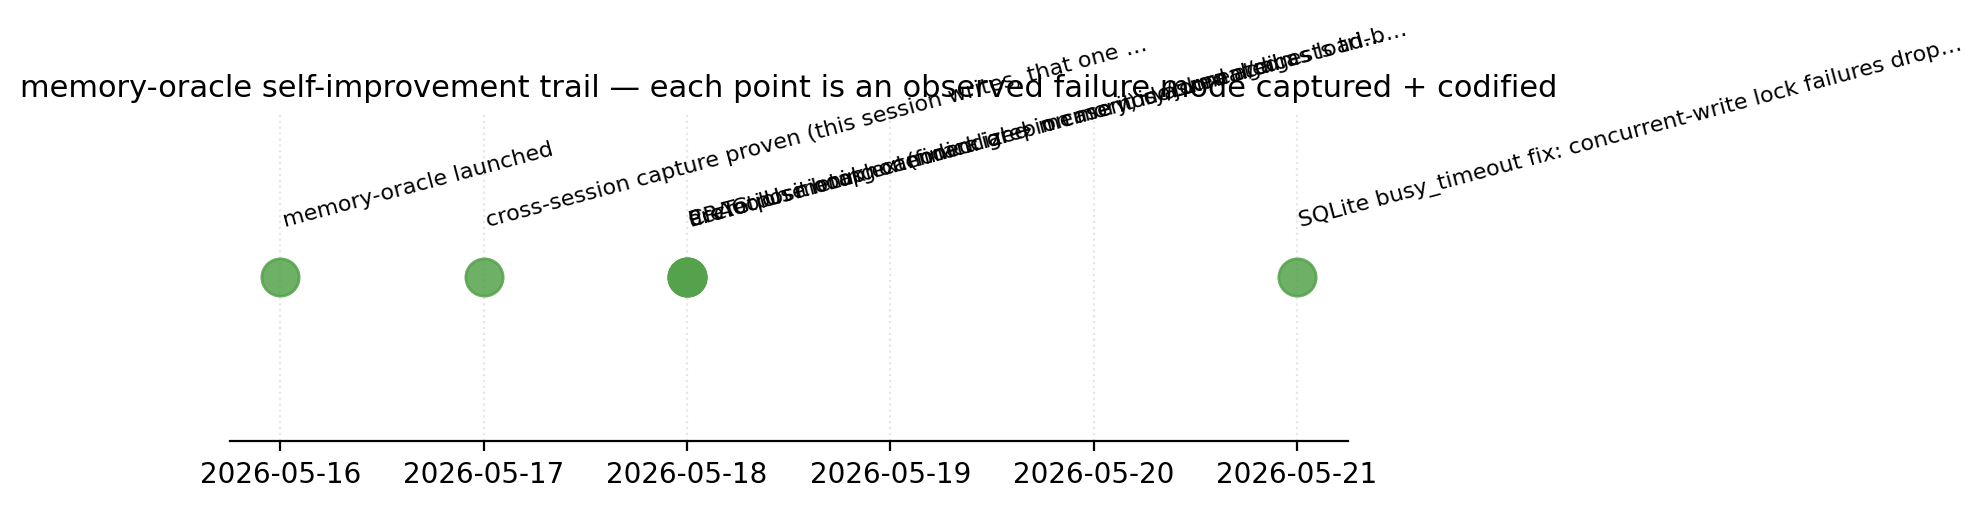
\includegraphics[width=0.95\textwidth]{../figures/F5-improvement-trail.png}
  \caption{Self-improvement trail. Each point is an observed failure
           captured as a memory file and codified as a change to the
           substrate or its operating procedure. All six improvements are
           themselves retrievable via \texttt{memory-search} --- the
           substrate's reflexivity makes its own learning legible to
           future sessions.}
  \label{fig:improvement}
\end{figure}

This pattern --- failure $\rightarrow$ memory $\rightarrow$ code change
$\rightarrow$ retrievable lesson --- is the practical instantiation of the
flywheel claim. The substrate is not merely \emph{used}; it is \emph{shaped}
by use, with full provenance.

\subsection{Three-Tier Retrieval Methodology}
\label{sec:tiers}

The substrate exposes three retrieval layers, each appropriate for a
different question class:

\begin{table}[h]
\centering
\caption{Three-tier retrieval. Each tier is appropriate for a different question class.}
\label{tab:tiers}
\small
\begin{tabular}{llll}
\toprule
\textbf{Tier} & \textbf{Tool} & \textbf{Target corpus} & \textbf{Best for} \\
\midrule
1   & \texttt{memory-search} (BM25 over FTS5) & Memory files + journal digests & Discovery (fast, ranked) \\
1.5 & Structural index (\texttt{surface\_map}) & Exact-string lookup over the indexed corpus & Precision (commands, paths) \\
2   & \texttt{memory-cite} (streamed JSONL) & Raw session transcripts & Forensic (verbatim at line/timestamp) \\
\bottomrule
\end{tabular}
\end{table}

Tiers compose: a fast Tier 1 hit saves the forensic Tier 2 cost. When
Tier 1 returns nothing, Tier 2 is still there. The PreToolUse hook
listed in Table~\ref{tab:components} auto-suggests Tier 1 when an agent
reaches for raw \texttt{grep} on memory directories --- closing a
recurrent failure mode in which agents skip the indexed digest layer
and conclude incorrectly that no prior decision exists.

\subsection{Lock-Contention Recovery}
\label{sec:contention}

Concurrent writes from multiple sessions exposed a SQLite lock contention
failure mode: roughly 47\% of write attempts during multi-session bursts
errored with \texttt{database is locked (5)} before fix. The mitigation
was to prepend the \texttt{.timeout 5000} dot-command to every
\texttt{sqlite3} CLI invocation in the watcher, which sets the per-connection
\texttt{busy\_timeout} to 5\,s at connection open --- importantly, this
must happen \emph{before} parse-time schema lookups, so the in-stdin
\texttt{PRAGMA} variant does not work; the dot-command does.

Post-fix, under 3 bursts of 10 concurrent writes each (30 total),
transient lock errors dropped to $\sim$10\% of attempts, with every file
ultimately landing in the index via the next watcher tick (FTS5 rebuild
is convergent). Net data loss: zero. This is documented to flag a class
of substrate-reliability work that has no precedent in vector-RAG systems
because they do not face the same write-concurrency profile: in our
substrate, every operator session is a potential writer.

% ============================================================================
\section{Discussion}
\label{sec:discussion}

\subsection{The Flywheel}

The system exhibits an emergent property we did not explicitly design: AI
agents primed with supersession-aware retrieval tend to author new memory
files during work. The fs-watcher absorbs these into the corpus; subsequent
sessions inherit them. This forms a \emph{flywheel}: the corpus extends
itself as a side-effect of being used, and the extensions are
provenance-preserving because new files start as canonical (and can later
be superseded if they prove inaccurate, without destroying the original).
We hypothesize that the flywheel is the long-run differentiator over
vector-RAG systems whose embeddings do not benefit from being read.

\subsection{Beyond Clinical}

The cross-domain generalization in Section~\ref{sec:cross-domain} suggests
the substrate applies to any domain with evolving rules, provenance
requirements, and stale-assertion risk. In particular, the implicit
supersession patterns we observed in an operator-curated trading platform
support the hypothesis that what current EHRs, trading platforms, legal
compliance systems, and incident-response runbooks all need is the same
primitive, surfaced explicitly.

\subsection{Limitations and Future Work}

(a) Authoring supersession sidecars requires deliberate clinician action;
automated detection of clinical-event boundaries from new notes (a clinical
NLP layer) would lower the authoring burden but introduce model-bias risk.
(b) BM25 ranking on clinical-vocabulary queries is partially mitigated by
the structural index for ICD codes and drug names; future work includes
clinical-vocabulary-aware tokenization. (c) Cross-jurisdiction patient
records (HIPAA / GDPR / PIPEDA) require additional governance design
beyond the cryptographic layer we present here.

% ============================================================================
\section{Conclusion}
\label{sec:conclusion}

We have introduced accretive supersession as a retrieval primitive for AI
agents in domains where stale assertions are dangerous, demonstrated it
end-to-end with a clinical case study and a cross-domain trading retrofit,
documented a trust model that places encryption keys with the patient
rather than the institution, and released the full reference implementation
under MIT license. The argument generalizes beyond clinical AI to any
domain where rules evolve in response to observed outcomes and provenance
matters. The reference implementation is operator-validated; the litmus
tests are reproducible from a single shell command.

The substrate we propose is not a new EHR. It is the memory layer underneath
every EHR, trading platform, and incident-response system---one that finally
treats corrections as first-class citizens of retrieval.

% ============================================================================
\bibliographystyle{splncs04}
\bibliography{references}

\end{document}
